\documentclass[10pt,a4paper]{amsart}
\usepackage[margin=19mm]{geometry}
\usepackage{amsmath,amssymb,mathtools}
\usepackage[scr=rsfs,cal=euler]{mathalfa}
\usepackage{xfrac}
\usepackage[unicode,hidelinks,bookmarks=false]{hyperref}
\newcommand{\ie}{i.e.\ }
\newcommand{\cf}{cf.\ }
\newcommand{\resp}{respectively\ }
\newcommand{\Subsection}{\subsection}
\providecommand{\nobreakdash}{\nobreak\hbox{-}}
\setlength{\emergencystretch}{2em}
\multlinegap0pt
\usepackage{mathtools}
\usepackage{enumitem}
\usepackage{tikz-cd}
\newtheorem{theorem}{Theorem}[section]
\newtheorem{lemma}[theorem]{Lemma}
\newtheorem{proposition}[theorem]{Proposition}
\newtheorem{corollary}[theorem]{Corollary}
\numberwithin{equation}{section}
\newtheorem{definition}[theorem]{Definition}
\newtheorem{remark}[theorem]{Remark}
\newcommand{\Z}{\mathbb Z}
\newcommand{\R}{\mathbb R}
\newcommand{\C}{\mathbb C}
\renewcommand{\P}{\mathbb P}
\newcommand{\cO}{\mathcal O}
\newcommand{\cR}{\mathcal R}
\newcommand{\CP}{\mathbb{CP}}
\newcommand{\wideand}{ \quad \text{ and } \quad }
\DeclareMathOperator{\cone}{cone}
\DeclareMathOperator{\link}{lk}
\DeclareMathOperator{\SO}{SO}
\DeclareMathOperator{\PD}{PD}
\DeclareMathOperator{\sign}{sign}
\DeclareMathOperator{\id}{id}
\DeclareMathOperator{\Int}{Int}
\begin{document}
\title[Cohomological rigidity of smooth toric Fano fourfolds]{Cohomological rigidity of smooth toric Fano fourfolds}
\author{Suyoung Choi}
\date{}
\maketitle
\noindent\emph{Source and licence.} Cohomological rigidity of smooth toric Fano fourfolds. Version arXiv:2608.17233v1 (CC BY 4.0). This material is distributed under the Creative Commons Attribution 4.0 International licence, http://creativecommons.org/licenses/by/4.0/, as recorded in the arXiv OAI licence metadata for this exact version and shown on the abstract page https://arxiv.org/abs/2608.17233v1. Full rights notice: licenses/arxiv-2608.17233-CC-BY-4.0.txt.\par\smallskip
\noindent\textit{Editorial scope.} Counted unit: the original \texttt{theorem} environment \texttt{thm:criterion\_flip} at source lines 474--478 together with its complete proof at lines 479--482; the delivered document keeps source lines 79--559 so that every referenced label and every citation resolves inside it. Native editable source is the paper's own concatenated TeX; the AMS wrapper is editorial formatting only. No publisher class, upstream script or unrelated artwork is redistributed.
\begin{theorem} \label{thm:main}
    The toric manifolds $X_{50}$ and $X_{57}$ are orientation-preservingly diffeomorphic.
\end{theorem}

Together with the classification results of~\cite{Higashitani-Kurimoto-Masuda2022}, the theorem completes the cohomological rigidity problem for smooth toric Fano fourfolds.

\begin{corollary}
    Any two smooth toric Fano fourfolds are diffeomorphic if their integral cohomology rings are isomorphic as graded rings.
\end{corollary}


\section{The Bott manifolds}\label{sec:fan-bott}

After an appropriate relabeling of the rays and a unimodular change of lattice basis\footnote{Relative to the ray ordering in \cite[Table~27]{Higashitani-Kurimoto-Masuda2022}, the new orders are $(1,3,4,2,5,6,7,8)$ for $X_{50}$ and $(1,3,4,2,5,6,8,7)$ for $X_{57}$. The new lattice basis is $(e_1,e_3,e_4,e_2)$ in terms of the basis used there.}, we may write the fans of $X_{50}$ and $X_{57}$ as follows:
\begin{align*}
    v_1&=e_1,& v_2&=e_2,& v_3&=e_3,& v_4&=e_4,\\
    v_5&=-e_1+e_2+e_3-e_4,& v_6&=-e_2+e_4,& v_8&=-e_4,
\end{align*}
together with
$$
    v_7^{50}=-e_3+e_4 \wideand v_7^{57}=-e_3.
$$
We label each ray by the index of its primitive generator. 
For a subset $I=\{i_1,\ldots,i_k\}\subset \{1,\ldots,8\}$, we write $i_1\cdots i_k$ for $I$. 
Whenever $\sigma_I \coloneq \cone(v_j\mid j\in I)$ is a cone of the fan under consideration, let $V(I)$ denote the closure of the corresponding torus orbit. 
In particular, $D_j \coloneq V(j)$ is the torus-invariant prime divisor corresponding to the ray $\R_{\geq 0}v_j$.
With these conventions, the two fans have the same minimal nonfaces
$$
    26,\quad 37,\quad 48,\quad 145,\quad 156,\quad 157, \wideand 238.
$$
For each $i\in\{50,57\}$, let $\Sigma_i$ denote the fan of $X_i$, and $\Sigma_i^-$ the fan with primitive ray generators $v_1$, $\ldots$, $v_6$, $v_7^i$, and $v_8$ whose underlying simplicial complex is the cross-polytope complex with minimal nonfaces
\begin{equation}\label{eq:B-mnf}
    15,\quad 26,\quad 37, \wideand 48.
\end{equation}
The ray generators are in the standard triangular form of a four-stage Bott fan. 
Hence $\Sigma_i^-$ is smooth and complete. 
We denote the associated Bott manifold by~$B_i$.
For background on Bott manifolds, see, for example, \cite{Grossberg-Karshon1994, Masuda-Panov2008,Choi-Hwang-Jang2025}.

For a finite set $I$, let $\Delta_I$ denote the simplex with vertex set $I$. 
The underlying simplicial complexes of $\Sigma_i^-$ and $\Sigma_i$ differ only by the local bistellar move
$$
    \Delta_{238}*\partial\Delta_{15} \quad\longleftrightarrow\quad \partial\Delta_{238}*\Delta_{15}.
$$
Equivalently, at the level of simplices, this move replaces 
\begin{equation}\label{eq:bistellar}
    \{1238,2358\} \quad\longleftrightarrow\quad \{1235,1258,1358\}.
\end{equation}
This is the $2$--$3$ bistellar move shown in Figure~\ref{fig:bistellar}.
\begin{figure}[t]
    \centering
    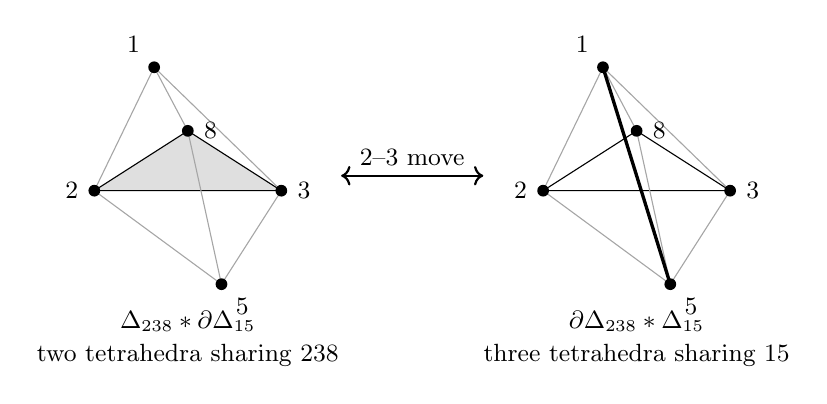
\begin{tikzpicture}[
        scale=0.95,
        vertex/.style={circle,fill=black,inner sep=1.5pt},
        every node/.style={font=\small}
    ]
        % Two tetrahedra
        \begin{scope}
            \coordinate (a2) at (-1.25,0);
            \coordinate (a3) at (1.25,0);
            \coordinate (a8) at (0,0.8);
            \coordinate (a1) at (-0.45,1.65);
            \coordinate (a5) at (0.45,-1.25);
        
            \fill[gray!25] (a2)--(a3)--(a8)--cycle;
            \draw (a2)--(a3)--(a8)--cycle;
            \foreach \x in {a2,a3,a8} {
                \draw[gray!70] (a1)--(\x);
                \draw[gray!70] (a5)--(\x);
            }
        
            \node[vertex,label=left:$2$] at (a2) {};
            \node[vertex,label=right:$3$] at (a3) {};
            \node[vertex,label=right:$8$] at (a8) {};
            \node[vertex,label=above left:$1$] at (a1) {};
            \node[vertex,label=below right:$5$] at (a5) {};
        
            \node at (0,-1.75) {$\Delta_{238}*\partial\Delta_{15}$};
            \node at (0,-2.2) {two tetrahedra sharing $238$};
        \end{scope}
        
        \draw[<->,thick] (2.05,0.2)--(3.95,0.2) node[midway,above] {$2$--$3$ move};
        
        % Three tetrahedra
        \begin{scope}[xshift=6cm]
            \coordinate (b2) at (-1.25,0);
            \coordinate (b3) at (1.25,0);
            \coordinate (b8) at (0,0.8);
            \coordinate (b1) at (-0.45,1.65);
            \coordinate (b5) at (0.45,-1.25);
        
            \draw (b2)--(b3)--(b8)--cycle;
            \foreach \x in {b2,b3,b8} {
                \draw[gray!70] (b1)--(\x);
                \draw[gray!70] (b5)--(\x);
            }
            \draw[very thick] (b1)--(b5);
        
            \node[vertex,label=left:$2$] at (b2) {};
            \node[vertex,label=right:$3$] at (b3) {};
            \node[vertex,label=right:$8$] at (b8) {};
            \node[vertex,label=above left:$1$] at (b1) {};
            \node[vertex,label=below right:$5$] at (b5) {};
        
            \node at (0,-1.75) {$\partial\Delta_{238}*\Delta_{15}$};
            \node at (0,-2.2) {three tetrahedra sharing $15$};
        \end{scope}
    \end{tikzpicture}
    \caption{The local $2$--$3$ bistellar move. The shaded face on the left and the thick edge on the right lie in the interior of the triangular bipyramid.}
    \label{fig:bistellar}
\end{figure}
The corresponding primitive relation is
$$
    v_0 \coloneq v_1+v_5=v_2+v_3+v_8=(0,1,1,-1).
$$

\begin{proposition}\label{prop:common-flip}
    For each $i\in\{50,57\}$, the toric manifold $X_i$ is obtained from~$B_i$ by the standard flip corresponding to the above $2$--$3$ bistellar move.
    The centers in~$B_i$ and $X_i$ are $C_i=V(238)\cong\CP^1$ and $V(15)\cong\CP^2$, respectively.
    Moreover,
    $$
        \nu_{C_i/B_i}\cong\cO_{\CP^1}(-1)^{\oplus3}.
    $$
\end{proposition}
\begin{proof}
    Since $v_0=v_2+v_3+v_8=v_1+v_5$, the star subdivisions of $\Sigma_i^-$ at $238$ and of $\Sigma_i$ at $15$, both with new ray $\R_{\geq0}v_0$, give the same fan.
    Thus the corresponding modification from $B_i$ to $X_i$ is the standard flip, with centers $V(238)\cong\CP^1$ and $V(15)\cong\CP^2$ on the two sides.

    The wall relation associated with $C_i$ is $v_1+v_5-v_2-v_3-v_8=0$.
    Hence
    $$
        D_2\cdot C_i=D_3\cdot C_i=D_8\cdot C_i=-1.
    $$
    Since $C_i=D_2\cap D_3\cap D_8$ transversely, it follows that
    $$
        \nu_{C_i/B_i} \cong \cO(D_2)|_{C_i}\oplus \cO(D_3)|_{C_i}\oplus \cO(D_8)|_{C_i} \cong \cO_{\CP^1}(-1)^{\oplus3}.
    $$
\end{proof}

Set $x=[D_5]$, $y=[D_6]$, $z=[D_7]$, and $u=[D_8]$.
The standard presentation of the cohomology ring of a smooth toric manifold~with \eqref{eq:B-mnf} gives
\begin{align*}
    H^\ast(B_{50};\Z) &\cong \frac{\Z[x,y,z,u]}{(x^2, y(y-x), z(z-x), u(u+x-y-z))}, \wideand\\
    H^\ast(B_{57};\Z) &\cong \frac{\Z[x,y,z,u]}{(x^2, y(y-x), z(z-x), u(u+x-y))}.
\end{align*}
All four generators have degree two.
Let $\psi\colon H^\ast(B_{50};\Z)\to H^\ast(B_{57};\Z)$ be a homomorphism defined by 
$$
    \psi(x)=-x+2z, \quad \psi(y)=z, \quad \psi(z)=z-y, \wideand \psi(u)=-u.
$$
A direct check shows that this assignment defines a graded ring isomorphism.
In both rings, $xyzu$ is the positive generator of~$H^8(B_i;\Z)$ determined by the complex orientation. 
Since $\psi(xyzu)=(-x+2z)z(z-y)(-u)=xyzu$, $\psi$ preserves the complex orientation.

Since $\PD[C_i]=[D_2][D_3][D_8]=(y-x)(z-x)u$, we obtain
\begin{equation}\label{eq:center-sign}
    \psi\bigl(\PD[C_{50}]\bigr) =-\PD[C_{57}].
\end{equation}

Strong cohomological rigidity of Bott manifolds says that every integral graded cohomology-ring isomorphism between Bott manifolds is induced by a diffeomorphism~\cite[Theorem~1.1]{Choi-Hwang-Jang2025}. 
Therefore there is an orientation-preserving diffeomorphism~$\Phi_0\colon B_{57}\to B_{50}$ such that $\Phi_0^*=\psi$.
By~\eqref{eq:center-sign} and Poincar\'e duality, 
\begin{equation}\label{eq:homology-sign} 
    (\Phi_0)_*[C_{57}]=-[C_{50}]. 
\end{equation}


\section{Construction of a diffeomorphism} \label{sec:transport}

We first describe the local model of the flip. 
Let $V=\C^2$ and $W=\C^3$, and let~$\gamma_V$ and~$\gamma_W$ be the tautological line bundles over $\P(V)=\CP^1$ and $\P(W)=\CP^2$, respectively. 
Put
$$
    E_V\coloneq \gamma_V\otimes W \cong \cO_{\CP^1}(-1)^{\oplus3}  \wideand E_W \coloneq V\otimes\gamma_W \cong \cO_{\CP^2}(-1)^{\oplus 2}.
$$
Equip $V$ and $W$ with conjugation-invariant Hermitian metrics.
Let $U(V)$ and~$U(W)$ denote their groups of complex-linear isometries.
We use the induced norm on~$V\otimes W$.

The complements of the zero sections in $E_V$ and $E_W$ are canonically identified with the space of nonzero rank-one tensors in $V\otimes W$. 
Indeed, a nonzero rank-one tensor $\xi$ determines unique lines $\ell\subset V$ and $m\subset W$. 
This gives a canonical $U(V)\times U(W)$-equivariant diffeomorphism $\chi\colon E_V\setminus\P(V)\to E_W\setminus\P(W)$ defined by~$\chi(\ell,\xi)=(m,\xi)$.
With respect to the tensor-product norm, $\chi$ preserves the norm and therefore restricts, for every $\varepsilon>0$, to a diffeomorphism
$$
    \chi_\varepsilon\colon \partial D_\varepsilon(E_V)\longrightarrow \partial D_\varepsilon(E_W).
$$

Let $S(V)$ and $S(W)$ denote the unit spheres in $V$ and $W$. 
The free circle action on $S(V)\times S(W)$ given by $\lambda\cdot(v,w)=(\lambda v,\lambda^{-1}w)$ yields $U(V)\times U(W)$-equivariant diffeomorphisms
$$
    \partial D_\varepsilon(E_V) \xleftarrow[\cong]{\alpha_V} \frac{S(V)\times S(W)}{S^1} \xrightarrow[\cong]{\alpha_W}\partial D_\varepsilon(E_W),
$$
where $\alpha_V([v,w])=([v],\varepsilon v\otimes w)$ and $\alpha_W([v,w])=([w],\varepsilon v\otimes w)$.
Since $S(V)\cong S^3$ and $S(W)\cong S^5$, both boundaries are equivariantly diffeomorphic to $\frac{S^3\times S^5}{S^1}$. 
Moreover, $\chi_\varepsilon=\alpha_W\circ\alpha_V^{-1}$.
Thus, on the underlying smooth manifolds, the standard flip replaces $D_\varepsilon(E_V)$ by $D_\varepsilon(E_W)$ along this common boundary identification \cite[Section~3.1]{Fu-Hoskins-PLehalleur2023}.

Complex conjugation on $S(V)\times S(W)$ descends to the involution $[v,w]\mapsto[\overline v,\overline w]$ on the common quotient. 
It induces involutions
$$
    J_V(\ell,\xi)=(\overline{\ell},\overline{\xi}) \wideand J_W(m,\xi)=(\overline{m},\overline{\xi}).
$$
The definition of $\chi$ gives $\chi\circ J_V=J_W\circ\chi$ on $E_V\setminus\P(V)$. 
In particular,
\begin{equation}\label{eq:conjugation}
    \chi_\varepsilon\circ J_V=J_W\circ\chi_\varepsilon.
\end{equation}


Now let us prove our main theorem.
\begin{proof}[Proof of Theorem~\ref{thm:main}]
    Let $\Phi_0\colon B_{57}\to B_{50}$ be the orientation-preserving diffeomorphism obtained in Section~\ref{sec:fan-bott}.
    We will modify $\Phi_0$ by isotopies so that it becomes compatible with the local model of the flip. 

    First, we isotope $\Phi_0$ to a diffeomorphism $\Phi_1\colon B_{57}\to B_{50}$ that maps $C_{57}$ to~$C_{50}$ as complex conjugation. 
    For each $i\in\{50,57\}$, choose a tubular neighborhood embedding $\tau_i\colon D_{\varepsilon_0}(E_V)\to B_i$ compatible with the standard local model above, and let
    $$
        \iota_i\coloneq \left.\tau_i\right|_{\P(V)} \colon \CP^1\longrightarrow C_i\subset B_i.
    $$
    We choose these local identifications so that $\iota_i$ preserves the complex orientation. 
    Let $c\colon\CP^1\to\CP^1$ be complex conjugation.
    By \eqref{eq:homology-sign},
    $$
        (\Phi_0\circ\iota_{57})_*[\CP^1] = -[C_{50}]= (\iota_{50}\circ c)_*[\CP^1] \in H_2(B_{50};\Z).
    $$
    Since the Bott manifold $B_{50}$ is simply connected, the Hurewicz map $\pi_2(B_{50})\to H_2(B_{50};\Z)$ is an isomorphism. 
    Hence the embeddings~$\Phi_0\circ\iota_{57}$ and $\iota_{50}\circ c$ are homotopic.
    
    Since $\dim_\R B_{50}=8>2\dim_\R \CP^1+2$, the stable embedding theorem implies that these embeddings are isotopic~\cite[Proposition~II]{Mazur1963}. 
    By the isotopy extension theorem~\cite[Proposition~III]{Mazur1963}, this isotopy extends to an ambient isotopy $\Psi_t$ of $B_{50}$ with $\Psi_0 = \id_{B_{50}}$.
    Thus $\Phi_1 \coloneq \Psi_1 \circ \Phi_0$ is an orientation-preserving diffeomorphism isotopic to~$\Phi_0$ and satisfies $\Phi_1\circ\iota_{57}=\iota_{50}\circ c$.
    In particular, $\Phi_1(C_{57})=C_{50}$, and~$\Phi_1|_{C_{57}}=c$ in the chosen parametrizations. 
    
    Next, we show that the normal bundle map induced by $\Phi_1$ is homotopic to $J_V$, and then further isotope $\Phi_1$ to a diffeomorphism $\Phi\colon B_{57}\to B_{50}$ compatible with the local model of the flip.
    
    Identify both normal bundles with $E_V$ by means of the chosen tubular neighborhoods. 
    Under these identifications, let $A\colon E_V\to E_V$ be the normal bundle map induced by $d\Phi_1$. 
    Then $A$ is a real vector-bundle isomorphism covering $c$.
    Both $A$ and $J_V$ reverse the orientations of the real rank-six fibers. 
    Indeed, $A$ reverses the normal orientation because $\Phi_1$ preserves the ambient orientation while $c$ reverses the orientation of the center. 
    The map $J_V$ reverses the fiber orientation because complex conjugation on a complex three-dimensional vector space has orientation sign~$(-1)^3=-1$. 
    Consequently, $G\coloneq J_V^{-1}A$ is an orientation-preserving automorphism of the underlying real rank-six bundle covering $\id_{\CP^1}$.
    
    Choose a bundle metric on the underlying oriented real rank-six bundle.
    Fiberwise polar decomposition gives a homotopy from $G$ through orientation-preserving bundle automorphisms to an orthogonal bundle automorphism. 
    Such an automorphism is a section of the bundle of orientation-preserving orthogonal automorphisms of the fibers of $E_V$. 
    This bundle has fiber~$\SO(6)$ and a canonical identity section.
    Standard obstruction theory for sections \cite[Part~III]{Steenrod1999book} shows that the section determined by the orthogonal automorphism is homotopic to the identity section. 
    Indeed, the obstructions to a homotopy over~$S^2\times I$, relative to $S^2\times\partial I$, lie in
    $$
        H^{j+1}\bigl(S^2\times I,S^2\times\partial I;\pi_j(SO(6))\bigr)\cong H^j\bigl(S^2;\pi_j(SO(6))\bigr)
    $$
    for $j=0,1,2$. 
    These groups vanish because
    $$
    \pi_0(SO(6))=\pi_2(SO(6))=0 \wideand H^1(S^2;\pi_1(SO(6)))=0.
    $$
    Thus $G$ is homotopic to the identity through orientation-preserving bundle automorphisms.
    It follows that $A=J_VG$ is homotopic to $J_V$ through real bundle isomorphisms covering $c$.

    Fix such a homotopy $A_t\colon E_V\to E_V$ for $0\leq t\leq 1$ with $A_0=A$ and $A_1=J_V$.
    Since the fiberwise operator norms of $A_t$ are uniformly bounded on the compact space $\CP^1\times[0,1]$, one can choose $0<\varepsilon\leq\varepsilon_0$ so that $A_t\bigl(D_\varepsilon(E_V)\bigr) \subset D_{\varepsilon_0}(E_V)$ for every $t\in[0,1]$.
    
    Set $h_0 \coloneq  \left.\Phi_1\circ\tau_{57}\right|_{D_\varepsilon(E_V)}$, $h_A \coloneq\left.\tau_{50}\circ A\right|_{D_\varepsilon(E_V)}$, and $h_1 \coloneq\left.\tau_{50}\circ J_V\right|_{D_\varepsilon(E_V)}$.
    The embeddings $h_0$ and $h_A$ agree on the zero section and induce the same normal bundle map $A$. 
    By the uniqueness theorem for tubular neighborhoods~\cite[Chapter~4, Theorem~5.3]{Hirsch1976book}, they are isotopic relative to the zero section, after decreasing $\varepsilon$ if necessary.
    The family $\tau_{50}\circ A_t|_{D_\varepsilon(E_V)}$ is an isotopy from $h_A$ to $h_1$, also relative to the zero section.
    Thus,$h_0$ and $h_1$ are isotopic relative to the zero section.

    After concatenating these isotopies, the ambient tubular neighborhood theorem~\cite[Chapter~8, Theorem~1.8]{Hirsch1976book} gives an ambient isotopy~$\Theta_t$ of~$B_{50}$, supported in an arbitrarily small neighborhood of $C_{50}$, such that, after decreasing $\varepsilon$ further if necessary, $\Theta_1\circ\Phi_1\circ\tau_{57}=\tau_{50}\circ J_V$ on~$D_\varepsilon(E_V)$.
    Define $\Phi \coloneq \Theta_1\circ\Phi_1$.
    Then $\Phi$ is an orientation-preserving diffeomorphism isotopic to~$\Phi_0$, and
    \begin{equation}\label{eq:J_V}
        \Phi\circ\tau_{57} =\tau_{50}\circ J_V \quad\text{on }D_\varepsilon(E_V).
    \end{equation}

    Perform the flip on both $B_{57}$ and $B_{50}$ by replacing the chosen copies of~$D_\varepsilon(E_V)$ with~$D_\varepsilon(E_W)$. 
    This gives $X_{57}$ and $X_{50}$. 
    Define $F$ by using $\Phi$ on the complements of the removed disk bundles and $J_W$ on the inserted copies of~$D_\varepsilon(E_W)$.
    
    To verify the compatibility on the boundary, let $q\in\partial D_\varepsilon(E_V)$. 
    In $X_{57}$, the point~$\tau_{57}(q)$ on the boundary of the complement is identified with $\chi_\varepsilon(q)$ on the inserted disk bundle. By
    \eqref{eq:conjugation} and \eqref{eq:J_V},
    $$
        J_W\bigl(\chi_\varepsilon(q)\bigr)=\chi_\varepsilon\bigl(J_V(q)\bigr)=\chi_\varepsilon\bigl( \tau_{50}^{-1}\circ\Phi\circ\tau_{57}(q) \bigr).
    $$
    The right-hand side is precisely the image of $\Phi(\tau_{57}(q))$ under the boundary identification defining~$X_{50}$. 
    Hence the two definitions of $F$ agree on the common boundary.
    The identity $\chi\circ J_V=J_W\circ\chi$ and \eqref{eq:J_V} show that the two maps agree on a collar of the common boundary. 
    Hence they glue smoothly to a diffeomorphism~$F\colon X_{57}\to X_{50}$.

    Finally, since complex conjugation in complex dimension~$d$ has real orientation sign~$(-1)^d$ and the total space of $E_W$ has complex dimension four, $J_W$ preserves orientation. 
    Since $\Phi$ is also orientation-preserving, the glued diffeomorphism $F$ preserves orientation.
\end{proof}
The map $F$ constructed in Theorem~\ref{thm:main} is illustrated in Figure~\ref{fig:flip-surgery}.

\begin{figure}[t]
    \centering
    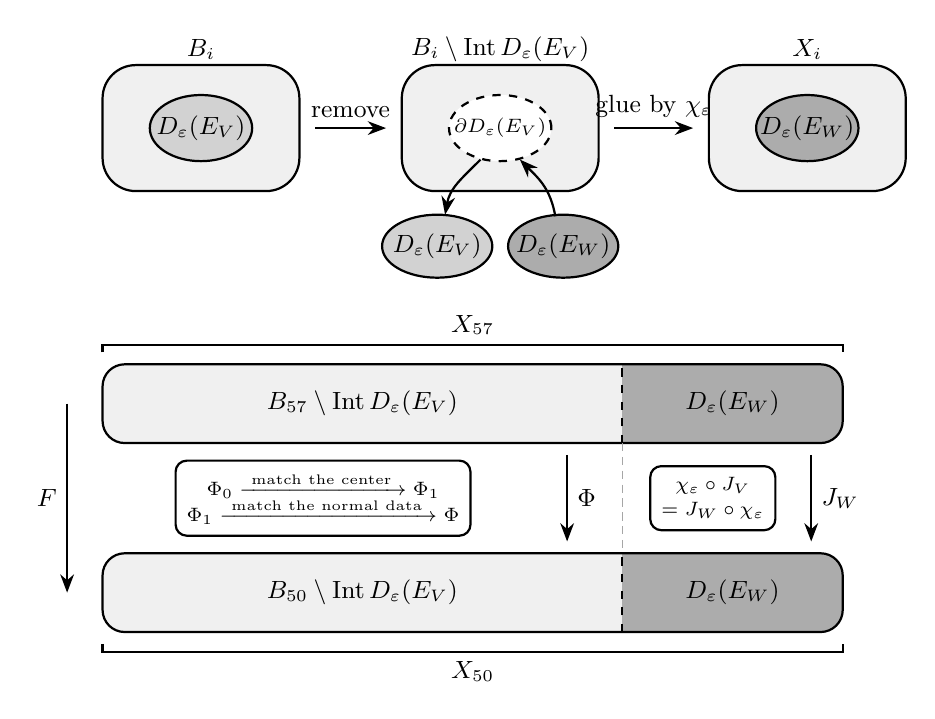
\begin{tikzpicture}[
        >=Stealth,
        every node/.style={font=\small},
        exterior/.style={draw, thick, rounded corners=12pt,fill=gray!12},
        oldpiece/.style={draw, thick, fill=gray!35},
        newpiece/.style={draw, thick, fill=gray!65},
        empty/.style={draw, thick, dashed, fill=white},
        roadmap/.style={draw, thick, rounded corners=4pt, fill=white, align=center, inner sep=4pt, font=\scriptsize}
    ]

    \draw[exterior] (0,1.5) rectangle (2.5,3.1);
    \draw[oldpiece] (1.25,2.3) ellipse [x radius=.65,y radius=.42];
    \node at (1.25,2.3) {$D_\varepsilon(E_V)$};
    \node at (1.25,3.3) {$B_i$};
    \draw[->,thick] (2.7,2.3) -- (3.6,2.3) node[midway,above] {remove};
    \draw[exterior] (3.8,1.5) rectangle (6.3,3.1);
    \draw[empty] (5.05,2.3) ellipse [x radius=.65,y radius=.42];
    \node[font=\scriptsize] at (5.05,2.3) {$\partial D_\varepsilon(E_V)$};
    \node at (5.05,3.3) {$B_i\setminus\operatorname{Int}D_\varepsilon(E_V)$};
    \draw[oldpiece] (4.25,.8) ellipse [x radius=.7,y radius=.4];
    \node at (4.25,.8) {$D_\varepsilon(E_V)$};
    \draw[->,thick] (4.8,1.9) to[out=225,in=80,looseness=1.05] (4.35,1.2);
    \draw[newpiece] (5.85,.8) ellipse [x radius=.7,y radius=.4];
    \node at (5.85,.8) {$D_\varepsilon(E_W)$};
    \draw[->,thick] (5.75,1.18) to[out=100,in=315,looseness=1.05] (5.3,1.9);
    \draw[->,thick] (6.5,2.3) -- (7.5,2.3) node[midway,above] {glue by $\chi_\varepsilon$};
    \draw[exterior] (7.7,1.5) rectangle (10.2,3.1);
    \draw[newpiece] (8.95,2.3) ellipse [x radius=.65,y radius=.42];
    \node at (8.95,2.3) {$D_\varepsilon(E_W)$};
    \node at (8.95,3.3) {$X_i$};

    \begin{scope}
        \clip[rounded corners=8pt] (0,-1.7) rectangle (9.4,-.7);
        \fill[gray!12] (0,-1.7) rectangle (9.4,-.7);
        \fill[gray!65] (6.6,-1.7) rectangle (9.4,-.7);
    \end{scope}

    \draw[thick,rounded corners=8pt] (0,-1.7) rectangle (9.4,-.7);
    \draw[thick,dashed] (6.6,-1.7) -- (6.6,-.7);
    \node at (3.3,-1.2) {$B_{57}\setminus \Int D_\varepsilon(E_V)$};
    \node at (8,-1.2) {$D_\varepsilon(E_W)$};
    \draw[thick] (0,-.55) -- (0,-.45) -- (9.4,-.45) -- (9.4,-.55);
    \node at (4.7,-.2) {$X_{57}$};

    \begin{scope}
        \clip[rounded corners=8pt] (0,-4.1) rectangle (9.4,-3.1);
        \fill[gray!12] (0,-4.1) rectangle (9.4,-3.1);
        \fill[gray!65] (6.6,-4.1) rectangle (9.4,-3.1);
    \end{scope}

    \draw[thick,rounded corners=8pt] (0,-4.1) rectangle (9.4,-3.1);
    \draw[thick,dashed] (6.6,-4.1) -- (6.6,-3.1);
    \node at (3.3,-3.6) {$B_{50}\setminus \Int D_\varepsilon(E_V)$};
    \node at (8,-3.6) {$D_\varepsilon(E_W)$};
    \node[roadmap] at (2.8,-2.4) { $\Phi_0 \xrightarrow{\;\text{match the center}\;} \Phi_1$ \\[-1pt] $\Phi_1 \xrightarrow{\;\text{match the normal data}\;} \Phi$};
    \draw[->,thick] (5.9,-1.85) -- (5.9,-2.95) node[midway,right] {$\Phi$};
    \draw[->,thick] (9,-1.85) -- (9,-2.95) node[midway,right] {$J_W$};
    \draw[->,thick] (-.45,-1.2) -- (-.45,-3.6) node[midway,left] {$F$};
    \draw[densely dashed,gray!70] (6.6,-1.7) -- (6.6,-3.1);
    \node[roadmap] at (7.75,-2.4) { $\chi_\varepsilon\circ J_V$\\[1pt]$=J_W\circ\chi_\varepsilon$ };

    \draw[thick] (0,-4.25) -- (0,-4.35) -- (9.4,-4.35) -- (9.4,-4.25);
    \node at (4.7,-4.6) {$X_{50}$};
    \end{tikzpicture}

    \caption{
        The flip replaces $D_\varepsilon(E_V)$ with $D_\varepsilon(E_W)$.
        Starting from the diffeomorphism~$\Phi_0\colon B_{57}\to B_{50}$, we obtain, through ambient isotopies, a diffeomorphism~$\Phi$ that agrees with the standard conjugation model on the tubular neighborhoods.
        The maps $\Phi$ on the complements and $J_W$ on the inserted disk bundles glue to form a diffeomorphism~$F\colon X_{57}\to X_{50}$.
    }
    \label{fig:flip-surgery}
\end{figure}


\section{Existence of diffeomorphisms across bistellar moves}

The proof of Theorem~\ref{thm:main} uses only the local model of a full-dimensional $2$--$(n-1)$ bistellar move. 
We record the resulting criterion.

Fix $n\ge 4$. 
For each $i\in\{0,1\}$, let $\Sigma_i^-$ and $\Sigma_i^+$ be smooth complete $n$-dimensional fans, and let $\cR_i$ denote their common set of rays.
Suppose that there are disjoint subsets $P_i,Q_i\subset\cR_i$ with 
$$
    |P_i|=2 \wideand |Q_i|=n-1,
$$
such that the underlying simplicial complex of $\Sigma_i^+$ is obtained from that of $\Sigma_i^-$ by the bistellar move
$$
    \Delta_{Q_i}*\partial\Delta_{P_i} \rightsquigarrow \partial\Delta_{Q_i}*\Delta_{P_i}.
$$
Assume also that
$$
    \sum_{\rho\in P_i}v_\rho =\sum_{\rho\in Q_i}v_\rho,
$$
where $v_\rho$ denotes the primitive generator of the ray $\rho$.

Set $B_i:=X_{\Sigma_i^-}$, $X_i:=X_{\Sigma_i^+}$, and $C_i:=V_{\Sigma_i^-}(Q_i)\cong\CP^1$.


\begin{theorem}\label{thm:criterion_flip}
    Suppose that there are a diffeomorphism~$\Phi\colon B_1\to B_0$ and a sign~$\varepsilon\in\{\pm1\}$ such that $\deg(\Phi)=\varepsilon^n$ and $\Phi_*[C_1]=\varepsilon[C_0]$.
    Then $\Phi$ is isotopic to a diffeomorphism compatible with the two flips. 
    Consequently, there is a diffeomorphism~$F\colon X_1\to X_0$ such that $\deg(F)=\deg(\Phi)=\varepsilon^n$.
\end{theorem}

\begin{proof}
    The proof is the same as that of Theorem~\ref{thm:main}, using the identity or complex conjugation on the standard local flip model according as $\varepsilon=1$ or $\varepsilon=-1$. 
    The assumption $n\ge 4$ gives the required stable embedding range.
\end{proof}


\begin{remark}
    Let $\omega_i\in H^{2n}(B_i;\Z)$ be the generator determined by the complex orientation, and set
    $$
        \alpha_i \coloneq \PD_{B_i}[C_i] = \prod_{\rho\in Q_i}[D_\rho] \in H^{2n-2}(B_i;\Z).
    $$
    Writing $\psi=\Phi^*$, the two sign conditions in Theorem~\ref{thm:criterion_flip} are equivalent to
    $$
        \psi(\omega_0)=\varepsilon^n\omega_1 \wideand \psi(\alpha_0)=\varepsilon^{n+1}\alpha_1.
    $$
    Thus, whenever the realizability of $\psi$ by a diffeomorphism is known, the remaining hypotheses can be checked from the fan data and the cohomology rings.
\end{remark}

\providecommand{\bysame}{\leavevmode\hbox to3em{\hrulefill}\thinspace}
\providecommand{\MR}{\relax\ifhmode\unskip\space\fi MR }
% \MRhref is called by the amsart/book/proc definition of \MR.
\providecommand{\MRhref}[2]{%
  \href{http://www.ams.org/mathscinet-getitem?mr=#1}{#2}
}
\providecommand{\href}[2]{#2}
\begin{thebibliography}{10}

\bibitem{Batyrev1999}
V.~V. Batyrev, \emph{On the classification of toric {F}ano {$4$}-folds},
  vol.~94, 1999, Algebraic geometry, 9, pp.~1021--1050. \MR{1703904}

\bibitem{Choi-Hwang-Jang2025}
Suyoung Choi, Taekgyu Hwang, and Hyeontae Jang, \emph{Strong cohomological
  rigidity of {B}ott manifolds}, Adv. Math. \textbf{473} (2025), Paper No.
  110305, 16. \MR{4899702}

\bibitem{Fu-Hoskins-PLehalleur2023}
Lie Fu, Victoria Hoskins, and Simon Pepin~Lehalleur, \emph{Motives of moduli
  spaces of bundles on curves via variation of stability and flips}, J. Lond.
  Math. Soc. (2) \textbf{108} (2023), no.~1, 1--53. \MR{4611824}

\bibitem{Grossberg-Karshon1994}
Michael Grossberg and Yael Karshon, \emph{Bott towers, complete integrability,
  and the extended character of representations}, Duke Math. J. \textbf{76}
  (1994), no.~1, 23--58. \MR{1301185}

\bibitem{Higashitani-Kurimoto-Masuda2022}
Akihiro Higashitani, Kazuki Kurimoto, and Mikiya Masuda, \emph{Cohomological
  rigidity for toric {F}ano manifolds of small dimensions or large {P}icard
  numbers}, Osaka J. Math. \textbf{59} (2022), no.~1, 177--215. \MR{4373489}

\bibitem{Hirsch1976book}
Morris~W. Hirsch, \emph{Differential topology}, Graduate Texts in Mathematics,
  vol. No. 33, Springer-Verlag, New York-Heidelberg, 1976. \MR{448362}

\bibitem{Masuda-Panov2008}
M.~Masuda and T.~E. Panov, \emph{Semi-free circle actions, {B}ott towers, and
  quasitoric manifolds}, Mat. Sb. \textbf{199} (2008), no.~8, 95--122.
  \MR{2452268}

\bibitem{Masuda-Suh2008}
Mikiya Masuda and Dong~Youp Suh, \emph{Classification problems of toric
  manifolds via topology}, Toric topology, Contemp. Math., vol. 460, Amer.
  Math. Soc., Providence, RI, 2008, pp.~273--286. \MR{2428362}

\bibitem{Mazur1963}
Barry Mazur, \emph{Differential topology from the point of view of simple
  homotopy theory}, Inst. Hautes \'Etudes Sci. Publ. Math. (1963), no.~15,
  5--93. \MR{161342}

\bibitem{Sato2000}
Hiroshi Sato, \emph{Toward the classification of higher-dimensional toric
  {F}ano varieties}, Tohoku Math. J. (2) \textbf{52} (2000), no.~3, 383--413.
  \MR{1772804}

\bibitem{Steenrod1999book}
Norman Steenrod, \emph{The topology of fibre bundles}, Princeton Landmarks in
  Mathematics, Princeton University Press, Princeton, NJ, 1999, Reprint of the
  1957 edition, Princeton Paperbacks. \MR{1688579}

\end{thebibliography}
\end{document}

\begin{thebibliography}{99}
\bibitem[Choi-Hwang-Jang2025]{Choi-Hwang-Jang2025} Suyoung Choi, Taekgyu Hwang, and Hyeontae Jang, \emph{Strong cohomological rigidity of {B}ott manifolds}, Adv. Math. \textbf{473} (2025), Paper No. 110305, 16. \MR{4899702}
\bibitem[Fu-Hoskins-PLehalleur2023]{Fu-Hoskins-PLehalleur2023} Lie Fu, Victoria Hoskins, and Simon Pepin~Lehalleur, \emph{Motives of moduli spaces of bundles on curves via variation of stability and flips}, J. Lond. Math. Soc. (2) \textbf{108} (2023), no.~1, 1--53. \MR{4611824}
\bibitem[Grossberg-Karshon1994]{Grossberg-Karshon1994} Michael Grossberg and Yael Karshon, \emph{Bott towers, complete integrability, and the extended character of representations}, Duke Math. J. \textbf{76} (1994), no.~1, 23--58. \MR{1301185}
\bibitem[Higashitani-Kurimoto-Masuda2022]{Higashitani-Kurimoto-Masuda2022} Akihiro Higashitani, Kazuki Kurimoto, and Mikiya Masuda, \emph{Cohomological rigidity for toric {F}ano manifolds of small dimensions or large {P}icard numbers}, Osaka J. Math. \textbf{59} (2022), no.~1, 177--215. \MR{4373489}
\bibitem[Hirsch1976book]{Hirsch1976book} Morris~W. Hirsch, \emph{Differential topology}, Graduate Texts in Mathematics, vol. No. 33, Springer-Verlag, New York-Heidelberg, 1976. \MR{448362}
\bibitem[Masuda-Panov2008]{Masuda-Panov2008} M.~Masuda and T.~E. Panov, \emph{Semi-free circle actions, {B}ott towers, and quasitoric manifolds}, Mat. Sb. \textbf{199} (2008), no.~8, 95--122. \MR{2452268}
\bibitem[Mazur1963]{Mazur1963} Barry Mazur, \emph{Differential topology from the point of view of simple homotopy theory}, Inst. Hautes \'Etudes Sci. Publ. Math. (1963), no.~15, 5--93. \MR{161342}
\bibitem[Steenrod1999book]{Steenrod1999book} Norman Steenrod, \emph{The topology of fibre bundles}, Princeton Landmarks in Mathematics, Princeton University Press, Princeton, NJ, 1999, Reprint of the 1957 edition, Princeton Paperbacks. \MR{1688579}
\end{thebibliography}
\end{document}
